% Creation
\section{Creation}
\subsection{Storing the project}
\begin{frame}{Storing the project}
    \begin{figure}
        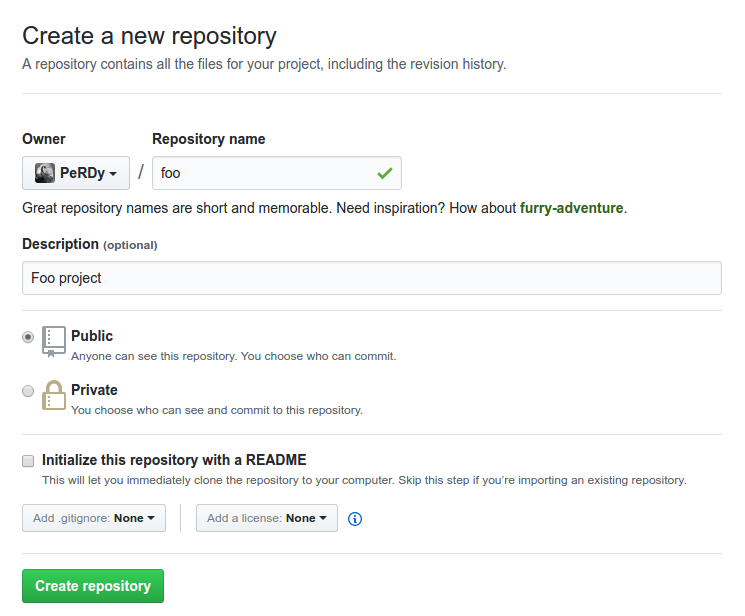
\includegraphics[width=\textwidth,height=0.8\textheight,keepaspectratio]{create_repository.png}
    \end{figure}
    \note{
        This speech is focused on open source, so working on GitHub.
    }
\end{frame}

\subsection{Create the project skeleton}
\begin{frame}[fragile]{Create the project skeleton}
    \begin{block}{Cookiecutter context}
        Define all variables needed by cookiecutter to properly create the project skeleton, these variables can be found in \textit{cookiecutter.json} file.
    \end{block}
    \pause
    \begin{block}{Create skeleton}
        Execute cookiecutter with previously defined context to create the project skeleton.
    \end{block}
    \pause
    \begin{block}{Commit \& push}
        Time to do your first commit and push to repository:
        \begin{minted}{bash}
git remote add origin git@github.com:PeRDy/foo.git
git commit -a -m "Initial commit"
git push
        \end{minted}
    \end{block}
\end{frame}

\subsection{Project hierarchy}
\begin{frame}{Project hierarchy}
    \begin{columns}
        \begin{column}{0.2\textwidth}
            \begin{figure}
                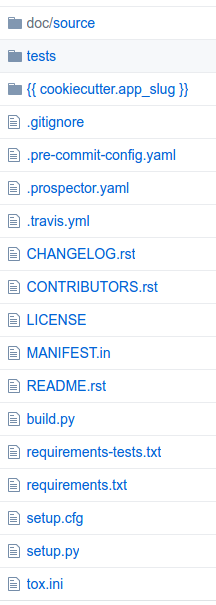
\includegraphics[width=\textwidth,height=\textheight,keepaspectratio]{project_skeleton.png}
            \end{figure}
        \end{column}
        \begin{column}{0.80\textwidth}
            \begin{block}{Documentation folder}
                The place that keeps all the documentation source files as well as the doc config file.
            \end{block}
            \pause
            \begin{block}{Tests folder}
                All tests files are stored in a tests folder where tests collectors can gather them without problems.
            \end{block}
            \pause
            \begin{block}{Application folder}
                The application itself, the \emph{python package} distributed, and the same that other users will import in their applications.
            \end{block}
            \pause
            \begin{block}{Root files}
                Files that keeps in the root directory are usually:
                \begin{itemize}
                    \item Tools configuration.
                    \item Services configuration.
                    \item Build scripts.
                    \item Metadata.
                \end{itemize}
            \end{block}
        \end{column}
    \end{columns}
    \note{
        \begin{description}
            \item[Tools configuration] Prospector, Pre-commit, Git.
            \item[Services configuration] Travis.
            \item[Build scripts] \texttt{build.py}, \texttt{setup.py}, \texttt{tox.ini}.
            \item[Metadata] Readme, manifest, contributors, changelog, requirements, \texttt{setup.cfg}.
        \end{description}
    }
\end{frame}

\begin{frame}{Relevant files I}
    \begin{block}{Manifest}
        This file, \texttt{MANIFEST.in}, with own syntax\footnote[1]{\href{https://docs.python.org/3/distutils/commandref.html#sdist-cmd}{https://docs.python.org/3/distutils/commandref.html#sdist-cmd}} defines the directories and files that will be included in the distributable package.
    \end{block}
    \pause
    \begin{block}{Requirements}
        List all requirements of your project, that are added as dependencies when installed. Usually requirements are splitted in two files: \texttt{requirements.txt} for real dependencies and \texttt{requirements-tests.txt} for dependencies necessaries to test the project.
    \end{block}
    \pause
    \begin{block}{Metadata}
        Metadata files: \texttt{README.rst}, \texttt{CONTRIBUTORS.rst}, \texttt{CHANGELOG.rst} and \texttt{LICENSE}.
    \end{block}
    \note{
        Readme can be written in rst or md, and will be the front page of the project in GitHub.
    }
\end{frame}

\begin{frame}{Relevant files II}
    \begin{block}{Tools and Services config}
        Configuration files for tools and services: \texttt{setup.cfg}, \texttt{.pre-commit-config.yaml}, \texttt{.prospector.yaml}, \texttt{.travis.yml}, \texttt{.gitignore}.
    \end{block}
    \pause
    \begin{block}{Setup}
        Main file that defines how the project will be packaged, gather metadata from other files and provides an interface to create distributable packages.
    \end{block}
    \pause
    \begin{block}{Tox}
        Tox file, \texttt{tox.ini}, defines the environments and commands that tox executes. In this case, defines an environment for each python version that should be tested, another for run lint tools and the last one for compile documentation.
    \end{block}
    \note{
        Main configuration file: \texttt{setup.cfg}. Ini-style file with sections for configuration of different tools, like \emph{bumpversion}, \emph{nose} and \emph{coverage}.

        Setup file keeps the requirements list, the current version, application name...

        Tox is integrated with travis.
    }
\end{frame}
\begin{frame}{Relevant files III}
    \begin{block}{Build}
        The build file, \texttt{build.py}, is the entrypoint for everything related to build, including \emph{testing}, \emph{packaging} and \emph{distributing}. This is a command line application using \emph{Clinner} that provides a set of utility commands such as:
        \begin{itemize}
            \item Run tests and code coverage.
            \item Run lint.
            \item Run tox.
            \item Create documentation.
            \item Upgrade version, create package and upload to pypi.
        \end{itemize}
    \end{block}
\end{frame}

\subsection{Bind services}
\begin{frame}{Bind Travis}
    \begin{figure}
        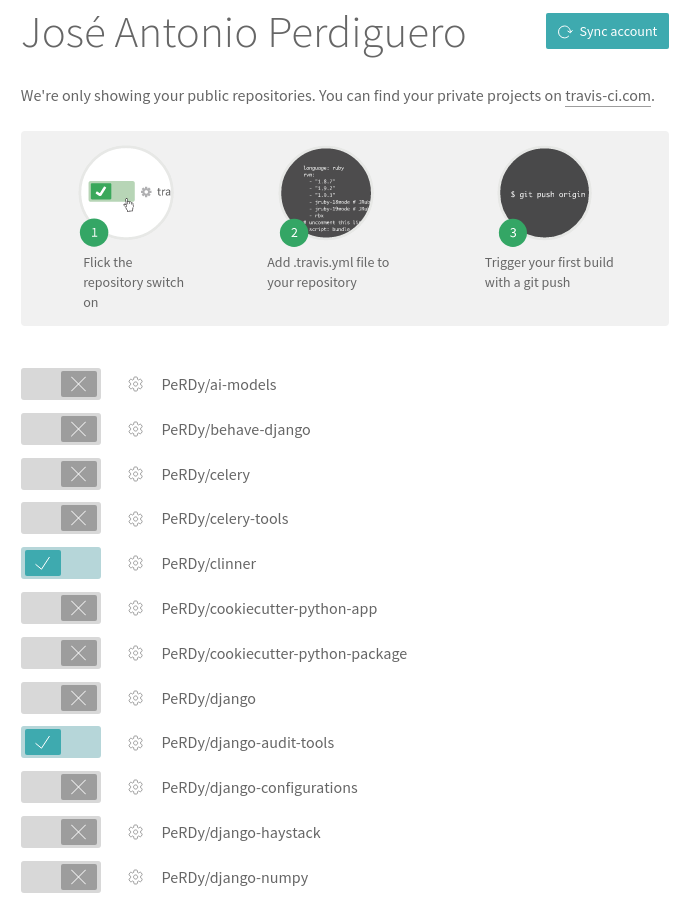
\includegraphics[width=\textwidth,height=0.8\textheight,keepaspectratio]{bind_travis.png}
    \end{figure}
\end{frame}
\begin{frame}{Bind Coveralls}
    \begin{figure}
        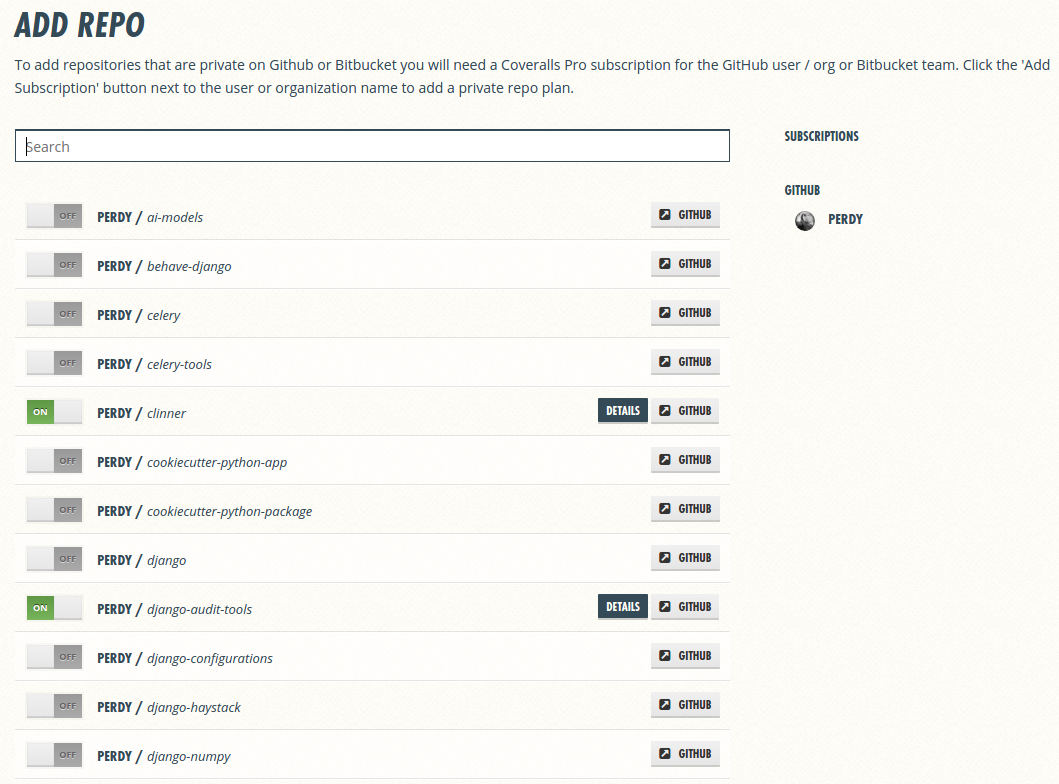
\includegraphics[width=\textwidth,height=0.8\textheight,keepaspectratio]{bind_coveralls.png}
    \end{figure}
\end{frame}
\begin{frame}{Bind ReadTheDocs}
    \begin{figure}
        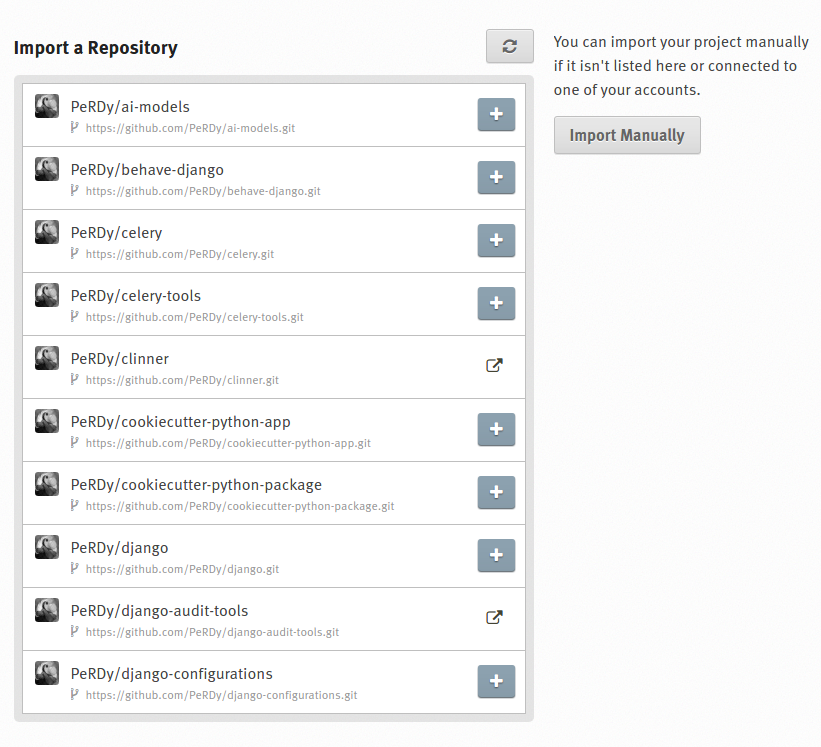
\includegraphics[width=\textwidth,height=0.8\textheight,keepaspectratio]{bind_readthedocs.png}
    \end{figure}
\end{frame}
